\documentclass{amsart}
\usepackage[margin=1in]{geometry}
\usepackage{amsmath,amsthm,amssymb}
\usepackage{graphicx,cleveref,array,capt-of,float,caption}
\usepackage{tikz}

\DeclareMathOperator{\area}{area}
\DeclareMathOperator{\dinv}{dinv}

\theoremstyle{definition}
\newtheorem{example}{Example}
\newtheorem{observation}{Observation}
\newtheorem{definition}{Definition}
\newtheorem{remark}{Remark}

\title{A plethora of valley data}
\begin{document}
\maketitle
\section{without assumption of $q,t$-symmetry}
We would like to find a bijection between standard parking functions with $k$ marked rises and standard parking functions with $k$ marked valleys.
\begin{example}
We tabulate all parking functions of semilength 3 with one marked rise/valley of area 1 as in \cref{fig:rise31,fig:val31}.
\begin{figure}[H]
\begin{minipage}[b]{0.49\textwidth}
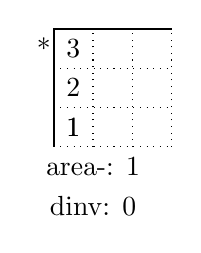
\begin{tikzpicture}[scale=0.5]
\draw[dotted] (0,0) grid (3,3);
\draw[thick] (0,0)--(0,1)--(0,2)--(0,3)--(1,3)--(2,3)--(3,3);
\draw node at (0.5,0.5) {1};
\draw node at (0.500000,0.500000) {1};
\draw node at (0.500000,1.500000) {2};
\draw node at (0.500000,2.500000) {3};
\draw node at (-0.250000,2.500000) {*};
\draw node at (1,-.5) {area-: 1};
\draw node at (1,-1.5) {dinv: 0};
\end{tikzpicture}
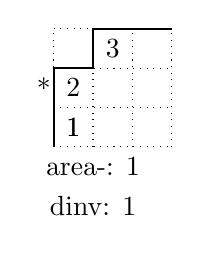
\begin{tikzpicture}[scale=0.5]
\draw[dotted] (0,0) grid (3,3);
\draw[thick] (0,0)--(0,1)--(0,2)--(1,2)--(1,3)--(2,3)--(3,3);
\draw node at (0.5,0.5) {1};
\draw node at (0.500000,0.500000) {1};
\draw node at (0.500000,1.500000) {2};
\draw node at (1.500000,2.500000) {3};
\draw node at (-0.250000,1.500000) {*};
\draw node at (1,-.5) {area-: 1};
\draw node at (1,-1.5) {dinv: 1};
\end{tikzpicture}
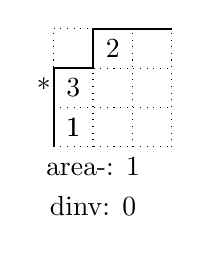
\begin{tikzpicture}[scale=0.5]
\draw[dotted] (0,0) grid (3,3);
\draw[thick] (0,0)--(0,1)--(0,2)--(1,2)--(1,3)--(2,3)--(3,3);
\draw node at (0.5,0.5) {1};
\draw node at (0.500000,0.500000) {1};
\draw node at (0.500000,1.500000) {3};
\draw node at (1.500000,2.500000) {2};
\draw node at (-0.250000,1.500000) {*};
\draw node at (1,-.5) {area-: 1};
\draw node at (1,-1.5) {dinv: 0};
\end{tikzpicture}
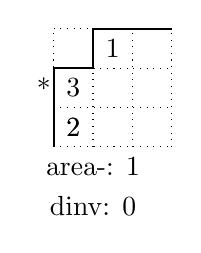
\begin{tikzpicture}[scale=0.5]
\draw[dotted] (0,0) grid (3,3);
\draw[thick] (0,0)--(0,1)--(0,2)--(1,2)--(1,3)--(2,3)--(3,3);
\draw node at (0.5,0.5) {2};
\draw node at (0.500000,0.500000) {2};
\draw node at (0.500000,1.500000) {3};
\draw node at (1.500000,2.500000) {1};
\draw node at (-0.250000,1.500000) {*};
\draw node at (1,-.5) {area-: 1};
\draw node at (1,-1.5) {dinv: 0};
\end{tikzpicture}
\captionof{figure}{Parking functions of 3 cars with one marked double rise and area 1.}
\label{fig:rise31}
\end{minipage}
\begin{minipage}[b]{0.49\textwidth}
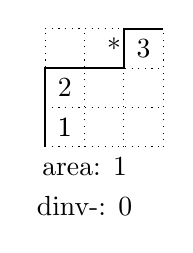
\begin{tikzpicture}[scale=0.5]
\draw[dotted] (0,0) grid (3,3);
\draw[thick] (0,0)--(0,1)--(0,2)--(1,2)--(2,2)--(2,3)--(3,3);
\draw node at (0.5,0.5) {1};
\draw node at (0.500000,0.500000) {1};
\draw node at (0.500000,1.500000) {2};
\draw node at (2.500000,2.500000) {3};
\draw node at (1.750000,2.500000) {*};
\draw node at (1,-.5) {area: 1};
\draw node at (1,-1.5) {dinv-: 0};
\end{tikzpicture}
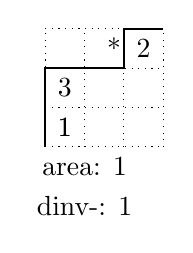
\begin{tikzpicture}[scale=0.5]
\draw[dotted] (0,0) grid (3,3);
\draw[thick] (0,0)--(0,1)--(0,2)--(1,2)--(2,2)--(2,3)--(3,3);
\draw node at (0.5,0.5) {1};
\draw node at (0.500000,0.500000) {1};
\draw node at (0.500000,1.500000) {3};
\draw node at (2.500000,2.500000) {2};
\draw node at (1.750000,2.500000) {*};
\draw node at (1,-.5) {area: 1};
\draw node at (1,-1.5) {dinv-: 1};
\end{tikzpicture}
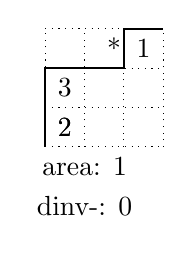
\begin{tikzpicture}[scale=0.5]
\draw[dotted] (0,0) grid (3,3);
\draw[thick] (0,0)--(0,1)--(0,2)--(1,2)--(2,2)--(2,3)--(3,3);
\draw node at (0.5,0.5) {2};
\draw node at (0.500000,0.500000) {2};
\draw node at (0.500000,1.500000) {3};
\draw node at (2.500000,2.500000) {1};
\draw node at (1.750000,2.500000) {*};
\draw node at (1,-.5) {area: 1};
\draw node at (1,-1.5) {dinv-: 0};
\end{tikzpicture}
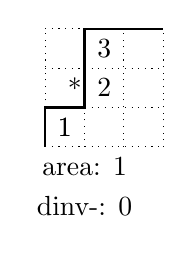
\begin{tikzpicture}[scale=0.5]
\draw[dotted] (0,0) grid (3,3);
\draw[thick] (0,0)--(0,1)--(1,1)--(1,2)--(1,3)--(2,3)--(3,3);
\draw node at (0.5,0.5) {1};
\draw node at (0.500000,0.500000) {1};
\draw node at (1.500000,1.500000) {2};
\draw node at (1.500000,2.500000) {3};
\draw node at (0.750000,1.500000) {*};
\draw node at (1,-.5) {area: 1};
\draw node at (1,-1.5) {dinv-: 0};
\end{tikzpicture}
\captionof{figure}{Parking functions of 3 cars with one marked valley and area 1.}
\label{fig:val31}
\end{minipage}
\end{figure}
\end{example}

\begin{example}
We tabulate all parking functions of semilength 4 with two marked rises/valleys with area 2 in \cref{fig:rise42,fig:val42}.
\begin{figure}[H]
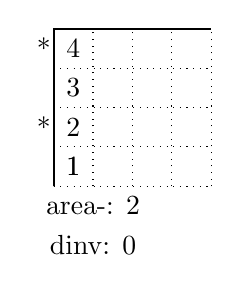
\begin{tikzpicture}[scale=0.5]
\draw[dotted] (0,0) grid (4,4);
\draw[thick] (0,0)--(0,1)--(0,2)--(0,3)--(0,4)--(1,4)--(2,4)--(3,4)--(4,4);
\draw node at (0.5,0.5) {1};
\draw node at (0.500000,0.500000) {1};
\draw node at (0.500000,1.500000) {2};
\draw node at (0.500000,2.500000) {3};
\draw node at (0.500000,3.500000) {4};
\draw node at (-0.250000,1.500000) {*};
\draw node at (-0.250000,3.500000) {*};
\draw node at (1,-.5) {area-: 2};
\draw node at (1,-1.5) {dinv: 0};
\end{tikzpicture}
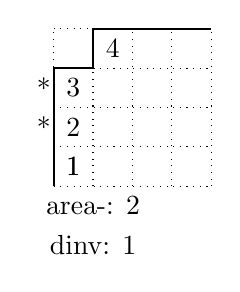
\begin{tikzpicture}[scale=0.5]
\draw[dotted] (0,0) grid (4,4);
\draw[thick] (0,0)--(0,1)--(0,2)--(0,3)--(1,3)--(1,4)--(2,4)--(3,4)--(4,4);
\draw node at (0.5,0.5) {1};
\draw node at (0.500000,0.500000) {1};
\draw node at (0.500000,1.500000) {2};
\draw node at (0.500000,2.500000) {3};
\draw node at (1.500000,3.500000) {4};
\draw node at (-0.250000,1.500000) {*};
\draw node at (-0.250000,2.500000) {*};
\draw node at (1,-.5) {area-: 2};
\draw node at (1,-1.5) {dinv: 1};
\end{tikzpicture}
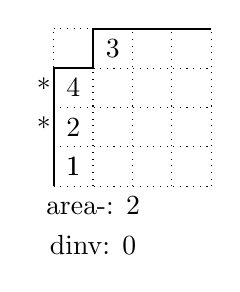
\begin{tikzpicture}[scale=0.5]
\draw[dotted] (0,0) grid (4,4);
\draw[thick] (0,0)--(0,1)--(0,2)--(0,3)--(1,3)--(1,4)--(2,4)--(3,4)--(4,4);
\draw node at (0.5,0.5) {1};
\draw node at (0.500000,0.500000) {1};
\draw node at (0.500000,1.500000) {2};
\draw node at (0.500000,2.500000) {4};
\draw node at (1.500000,3.500000) {3};
\draw node at (-0.250000,1.500000) {*};
\draw node at (-0.250000,2.500000) {*};
\draw node at (1,-.5) {area-: 2};
\draw node at (1,-1.5) {dinv: 0};
\end{tikzpicture}
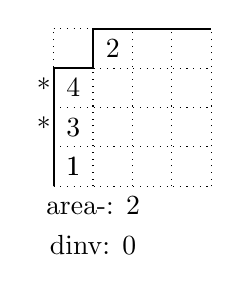
\begin{tikzpicture}[scale=0.5]
\draw[dotted] (0,0) grid (4,4);
\draw[thick] (0,0)--(0,1)--(0,2)--(0,3)--(1,3)--(1,4)--(2,4)--(3,4)--(4,4);
\draw node at (0.5,0.5) {1};
\draw node at (0.500000,0.500000) {1};
\draw node at (0.500000,1.500000) {3};
\draw node at (0.500000,2.500000) {4};
\draw node at (1.500000,3.500000) {2};
\draw node at (-0.250000,1.500000) {*};
\draw node at (-0.250000,2.500000) {*};
\draw node at (1,-.5) {area-: 2};
\draw node at (1,-1.5) {dinv: 0};
\end{tikzpicture}
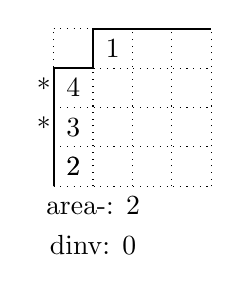
\begin{tikzpicture}[scale=0.5]
\draw[dotted] (0,0) grid (4,4);
\draw[thick] (0,0)--(0,1)--(0,2)--(0,3)--(1,3)--(1,4)--(2,4)--(3,4)--(4,4);
\draw node at (0.5,0.5) {2};
\draw node at (0.500000,0.500000) {2};
\draw node at (0.500000,1.500000) {3};
\draw node at (0.500000,2.500000) {4};
\draw node at (1.500000,3.500000) {1};
\draw node at (-0.250000,1.500000) {*};
\draw node at (-0.250000,2.500000) {*};
\draw node at (1,-.5) {area-: 2};
\draw node at (1,-1.5) {dinv: 0};
\end{tikzpicture}
\caption{Parking functions of semilength 4 with two marked rises and area 2.}
\label{fig:rise42}
\end{figure}
\begin{figure}[H]
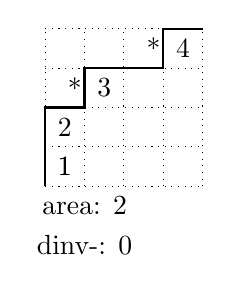
\begin{tikzpicture}[scale=0.5]
\draw[dotted] (0,0) grid (4,4);
\draw[thick] (0,0)--(0,1)--(0,2)--(1,2)--(1,3)--(2,3)--(3,3)--(3,4)--(4,4);
\draw node at (0.5,0.5) {1};
\draw node at (0.500000,0.500000) {1};
\draw node at (0.500000,1.500000) {2};
\draw node at (1.500000,2.500000) {3};
\draw node at (3.500000,3.500000) {4};
\draw node at (0.750000,2.500000) {*};
\draw node at (2.750000,3.500000) {*};
\draw node at (1,-.5) {area: 2};
\draw node at (1,-1.5) {dinv-: 0};
\end{tikzpicture}
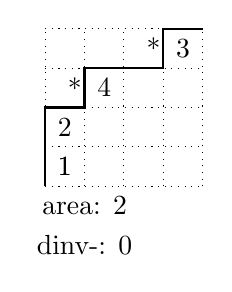
\begin{tikzpicture}[scale=0.5]
\draw[dotted] (0,0) grid (4,4);
\draw[thick] (0,0)--(0,1)--(0,2)--(1,2)--(1,3)--(2,3)--(3,3)--(3,4)--(4,4);
\draw node at (0.5,0.5) {1};
\draw node at (0.500000,0.500000) {1};
\draw node at (0.500000,1.500000) {2};
\draw node at (1.500000,2.500000) {4};
\draw node at (3.500000,3.500000) {3};
\draw node at (0.750000,2.500000) {*};
\draw node at (2.750000,3.500000) {*};
\draw node at (1,-.5) {area: 2};
\draw node at (1,-1.5) {dinv-: 0};
\end{tikzpicture}
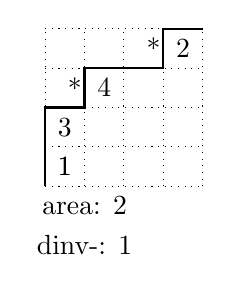
\begin{tikzpicture}[scale=0.5]
\draw[dotted] (0,0) grid (4,4);
\draw[thick] (0,0)--(0,1)--(0,2)--(1,2)--(1,3)--(2,3)--(3,3)--(3,4)--(4,4);
\draw node at (0.5,0.5) {1};
\draw node at (0.500000,0.500000) {1};
\draw node at (0.500000,1.500000) {3};
\draw node at (1.500000,2.500000) {4};
\draw node at (3.500000,3.500000) {2};
\draw node at (0.750000,2.500000) {*};
\draw node at (2.750000,3.500000) {*};
\draw node at (1,-.5) {area: 2};
\draw node at (1,-1.5) {dinv-: 1};
\end{tikzpicture}
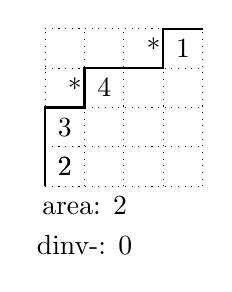
\begin{tikzpicture}[scale=0.5]
\draw[dotted] (0,0) grid (4,4);
\draw[thick] (0,0)--(0,1)--(0,2)--(1,2)--(1,3)--(2,3)--(3,3)--(3,4)--(4,4);
\draw node at (0.5,0.5) {2};
\draw node at (0.500000,0.500000) {2};
\draw node at (0.500000,1.500000) {3};
\draw node at (1.500000,2.500000) {4};
\draw node at (3.500000,3.500000) {1};
\draw node at (0.750000,2.500000) {*};
\draw node at (2.750000,3.500000) {*};
\draw node at (1,-.5) {area: 2};
\draw node at (1,-1.5) {dinv-: 0};
\end{tikzpicture}
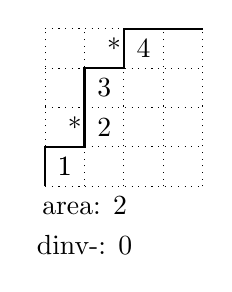
\begin{tikzpicture}[scale=0.5]
\draw[dotted] (0,0) grid (4,4);
\draw[thick] (0,0)--(0,1)--(1,1)--(1,2)--(1,3)--(2,3)--(2,4)--(3,4)--(4,4);
\draw node at (0.5,0.5) {1};
\draw node at (0.500000,0.500000) {1};
\draw node at (1.500000,1.500000) {2};
\draw node at (1.500000,2.500000) {3};
\draw node at (2.500000,3.500000) {4};
\draw node at (0.750000,1.500000) {*};
\draw node at (1.750000,3.500000) {*};
\draw node at (1,-.5) {area: 2};
\draw node at (1,-1.5) {dinv-: 0};
\end{tikzpicture}
\captionof{figure}{Parking functions of semilength 4 and two marked valleys and area 2}
\label{fig:val42}
\end{figure}
\end{example}

\begin{example}
We tabulate all parking functions of semilength 4 with two marked rises/valleys of area 1 in \cref{fig:rise421,fig:val421}.
\begin{figure}[H]
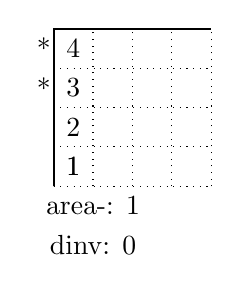
\begin{tikzpicture}[scale=0.5]
\draw[dotted] (0,0) grid (4,4);
\draw[thick] (0,0)--(0,1)--(0,2)--(0,3)--(0,4)--(1,4)--(2,4)--(3,4)--(4,4);
\draw node at (0.5,0.5) {1};
\draw node at (0.500000,0.500000) {1};
\draw node at (0.500000,1.500000) {2};
\draw node at (0.500000,2.500000) {3};
\draw node at (0.500000,3.500000) {4};
\draw node at (-0.250000,2.500000) {*};
\draw node at (-0.250000,3.500000) {*};
\draw node at (1,-.5) {area-: 1};
\draw node at (1,-1.5) {dinv: 0};
\end{tikzpicture}
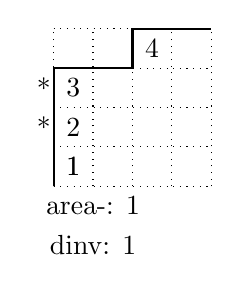
\begin{tikzpicture}[scale=0.5]
\draw[dotted] (0,0) grid (4,4);
\draw[thick] (0,0)--(0,1)--(0,2)--(0,3)--(1,3)--(2,3)--(2,4)--(3,4)--(4,4);
\draw node at (0.5,0.5) {1};
\draw node at (0.500000,0.500000) {1};
\draw node at (0.500000,1.500000) {2};
\draw node at (0.500000,2.500000) {3};
\draw node at (2.500000,3.500000) {4};
\draw node at (-0.250000,1.500000) {*};
\draw node at (-0.250000,2.500000) {*};
\draw node at (1,-.5) {area-: 1};
\draw node at (1,-1.5) {dinv: 1};
\end{tikzpicture}
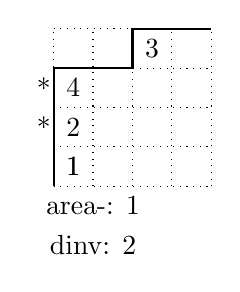
\begin{tikzpicture}[scale=0.5]
\draw[dotted] (0,0) grid (4,4);
\draw[thick] (0,0)--(0,1)--(0,2)--(0,3)--(1,3)--(2,3)--(2,4)--(3,4)--(4,4);
\draw node at (0.5,0.5) {1};
\draw node at (0.500000,0.500000) {1};
\draw node at (0.500000,1.500000) {2};
\draw node at (0.500000,2.500000) {4};
\draw node at (2.500000,3.500000) {3};
\draw node at (-0.250000,1.500000) {*};
\draw node at (-0.250000,2.500000) {*};
\draw node at (1,-.5) {area-: 1};
\draw node at (1,-1.5) {dinv: 2};
\end{tikzpicture}
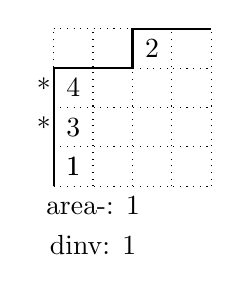
\begin{tikzpicture}[scale=0.5]
\draw[dotted] (0,0) grid (4,4);
\draw[thick] (0,0)--(0,1)--(0,2)--(0,3)--(1,3)--(2,3)--(2,4)--(3,4)--(4,4);
\draw node at (0.5,0.5) {1};
\draw node at (0.500000,0.500000) {1};
\draw node at (0.500000,1.500000) {3};
\draw node at (0.500000,2.500000) {4};
\draw node at (2.500000,3.500000) {2};
\draw node at (-0.250000,1.500000) {*};
\draw node at (-0.250000,2.500000) {*};
\draw node at (1,-.5) {area-: 1};
\draw node at (1,-1.5) {dinv: 1};
\end{tikzpicture}
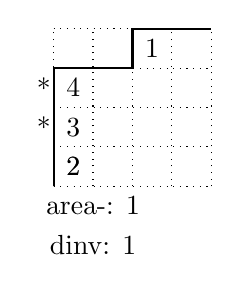
\begin{tikzpicture}[scale=0.5]
\draw[dotted] (0,0) grid (4,4);
\draw[thick] (0,0)--(0,1)--(0,2)--(0,3)--(1,3)--(2,3)--(2,4)--(3,4)--(4,4);
\draw node at (0.5,0.5) {2};
\draw node at (0.500000,0.500000) {2};
\draw node at (0.500000,1.500000) {3};
\draw node at (0.500000,2.500000) {4};
\draw node at (2.500000,3.500000) {1};
\draw node at (-0.250000,1.500000) {*};
\draw node at (-0.250000,2.500000) {*};
\draw node at (1,-.5) {area-: 1};
\draw node at (1,-1.5) {dinv: 1};
\end{tikzpicture}
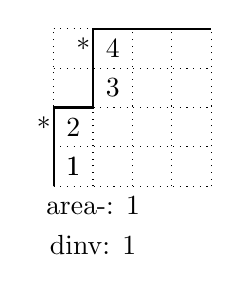
\begin{tikzpicture}[scale=0.5]
\draw[dotted] (0,0) grid (4,4);
\draw[thick] (0,0)--(0,1)--(0,2)--(1,2)--(1,3)--(1,4)--(2,4)--(3,4)--(4,4);
\draw node at (0.5,0.5) {1};
\draw node at (0.500000,0.500000) {1};
\draw node at (0.500000,1.500000) {2};
\draw node at (1.500000,2.500000) {3};
\draw node at (1.500000,3.500000) {4};
\draw node at (-0.250000,1.500000) {*};
\draw node at (0.750000,3.500000) {*};
\draw node at (1,-.5) {area-: 1};
\draw node at (1,-1.5) {dinv: 1};
\end{tikzpicture}
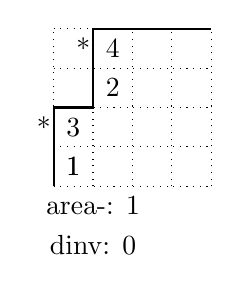
\begin{tikzpicture}[scale=0.5]
\draw[dotted] (0,0) grid (4,4);
\draw[thick] (0,0)--(0,1)--(0,2)--(1,2)--(1,3)--(1,4)--(2,4)--(3,4)--(4,4);
\draw node at (0.5,0.5) {1};
\draw node at (0.500000,0.500000) {1};
\draw node at (0.500000,1.500000) {3};
\draw node at (1.500000,2.500000) {2};
\draw node at (1.500000,3.500000) {4};
\draw node at (-0.250000,1.500000) {*};
\draw node at (0.750000,3.500000) {*};
\draw node at (1,-.5) {area-: 1};
\draw node at (1,-1.5) {dinv: 0};
\end{tikzpicture}
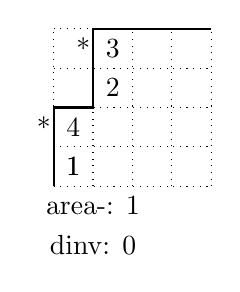
\begin{tikzpicture}[scale=0.5]
\draw[dotted] (0,0) grid (4,4);
\draw[thick] (0,0)--(0,1)--(0,2)--(1,2)--(1,3)--(1,4)--(2,4)--(3,4)--(4,4);
\draw node at (0.5,0.5) {1};
\draw node at (0.500000,0.500000) {1};
\draw node at (0.500000,1.500000) {4};
\draw node at (1.500000,2.500000) {2};
\draw node at (1.500000,3.500000) {3};
\draw node at (-0.250000,1.500000) {*};
\draw node at (0.750000,3.500000) {*};
\draw node at (1,-.5) {area-: 1};
\draw node at (1,-1.5) {dinv: 0};
\end{tikzpicture}
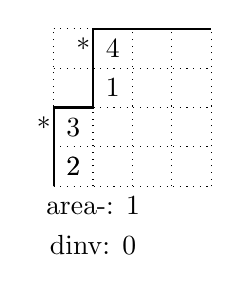
\begin{tikzpicture}[scale=0.5]
\draw[dotted] (0,0) grid (4,4);
\draw[thick] (0,0)--(0,1)--(0,2)--(1,2)--(1,3)--(1,4)--(2,4)--(3,4)--(4,4);
\draw node at (0.5,0.5) {2};
\draw node at (0.500000,0.500000) {2};
\draw node at (0.500000,1.500000) {3};
\draw node at (1.500000,2.500000) {1};
\draw node at (1.500000,3.500000) {4};
\draw node at (-0.250000,1.500000) {*};
\draw node at (0.750000,3.500000) {*};
\draw node at (1,-.5) {area-: 1};
\draw node at (1,-1.5) {dinv: 0};
\end{tikzpicture}
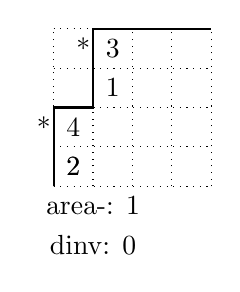
\begin{tikzpicture}[scale=0.5]
\draw[dotted] (0,0) grid (4,4);
\draw[thick] (0,0)--(0,1)--(0,2)--(1,2)--(1,3)--(1,4)--(2,4)--(3,4)--(4,4);
\draw node at (0.5,0.5) {2};
\draw node at (0.500000,0.500000) {2};
\draw node at (0.500000,1.500000) {4};
\draw node at (1.500000,2.500000) {1};
\draw node at (1.500000,3.500000) {3};
\draw node at (-0.250000,1.500000) {*};
\draw node at (0.750000,3.500000) {*};
\draw node at (1,-.5) {area-: 1};
\draw node at (1,-1.5) {dinv: 0};
\end{tikzpicture}
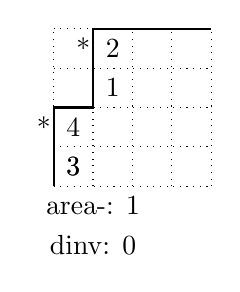
\begin{tikzpicture}[scale=0.5]
\draw[dotted] (0,0) grid (4,4);
\draw[thick] (0,0)--(0,1)--(0,2)--(1,2)--(1,3)--(1,4)--(2,4)--(3,4)--(4,4);
\draw node at (0.5,0.5) {3};
\draw node at (0.500000,0.500000) {3};
\draw node at (0.500000,1.500000) {4};
\draw node at (1.500000,2.500000) {1};
\draw node at (1.500000,3.500000) {2};
\draw node at (-0.250000,1.500000) {*};
\draw node at (0.750000,3.500000) {*};
\draw node at (1,-.5) {area-: 1};
\draw node at (1,-1.5) {dinv: 0};
\end{tikzpicture}
\caption{Parking functions of semilength 4 with two marked rises and area 1.}
\label{fig:rise421}
\end{figure}
\begin{figure}[H]
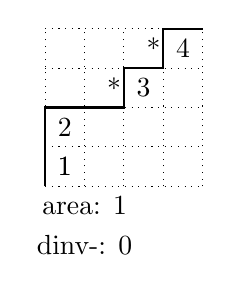
\begin{tikzpicture}[scale=0.5]
\draw[dotted] (0,0) grid (4,4);
\draw[thick] (0,0)--(0,1)--(0,2)--(1,2)--(2,2)--(2,3)--(3,3)--(3,4)--(4,4);
\draw node at (0.5,0.5) {1};
\draw node at (0.500000,0.500000) {1};
\draw node at (0.500000,1.500000) {2};
\draw node at (2.500000,2.500000) {3};
\draw node at (3.500000,3.500000) {4};
\draw node at (1.750000,2.500000) {*};
\draw node at (2.750000,3.500000) {*};
\draw node at (1,-.5) {area: 1};
\draw node at (1,-1.5) {dinv-: 0};
\end{tikzpicture}
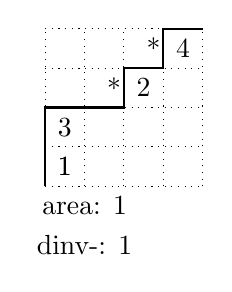
\begin{tikzpicture}[scale=0.5]
\draw[dotted] (0,0) grid (4,4);
\draw[thick] (0,0)--(0,1)--(0,2)--(1,2)--(2,2)--(2,3)--(3,3)--(3,4)--(4,4);
\draw node at (0.5,0.5) {1};
\draw node at (0.500000,0.500000) {1};
\draw node at (0.500000,1.500000) {3};
\draw node at (2.500000,2.500000) {2};
\draw node at (3.500000,3.500000) {4};
\draw node at (1.750000,2.500000) {*};
\draw node at (2.750000,3.500000) {*};
\draw node at (1,-.5) {area: 1};
\draw node at (1,-1.5) {dinv-: 1};
\end{tikzpicture}
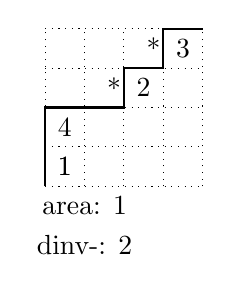
\begin{tikzpicture}[scale=0.5]
\draw[dotted] (0,0) grid (4,4);
\draw[thick] (0,0)--(0,1)--(0,2)--(1,2)--(2,2)--(2,3)--(3,3)--(3,4)--(4,4);
\draw node at (0.5,0.5) {1};
\draw node at (0.500000,0.500000) {1};
\draw node at (0.500000,1.500000) {4};
\draw node at (2.500000,2.500000) {2};
\draw node at (3.500000,3.500000) {3};
\draw node at (1.750000,2.500000) {*};
\draw node at (2.750000,3.500000) {*};
\draw node at (1,-.5) {area: 1};
\draw node at (1,-1.5) {dinv-: 2};
\end{tikzpicture}
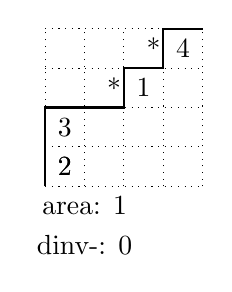
\begin{tikzpicture}[scale=0.5]
\draw[dotted] (0,0) grid (4,4);
\draw[thick] (0,0)--(0,1)--(0,2)--(1,2)--(2,2)--(2,3)--(3,3)--(3,4)--(4,4);
\draw node at (0.5,0.5) {2};
\draw node at (0.500000,0.500000) {2};
\draw node at (0.500000,1.500000) {3};
\draw node at (2.500000,2.500000) {1};
\draw node at (3.500000,3.500000) {4};
\draw node at (1.750000,2.500000) {*};
\draw node at (2.750000,3.500000) {*};
\draw node at (1,-.5) {area: 1};
\draw node at (1,-1.5) {dinv-: 0};
\end{tikzpicture}
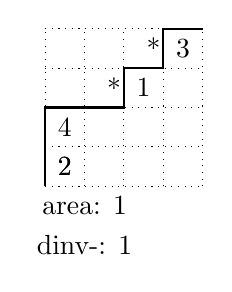
\begin{tikzpicture}[scale=0.5]
\draw[dotted] (0,0) grid (4,4);
\draw[thick] (0,0)--(0,1)--(0,2)--(1,2)--(2,2)--(2,3)--(3,3)--(3,4)--(4,4);
\draw node at (0.5,0.5) {2};
\draw node at (0.500000,0.500000) {2};
\draw node at (0.500000,1.500000) {4};
\draw node at (2.500000,2.500000) {1};
\draw node at (3.500000,3.500000) {3};
\draw node at (1.750000,2.500000) {*};
\draw node at (2.750000,3.500000) {*};
\draw node at (1,-.5) {area: 1};
\draw node at (1,-1.5) {dinv-: 1};
\end{tikzpicture}
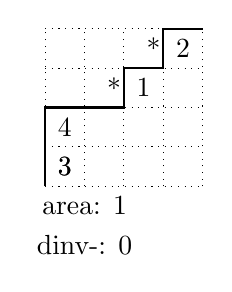
\begin{tikzpicture}[scale=0.5]
\draw[dotted] (0,0) grid (4,4);
\draw[thick] (0,0)--(0,1)--(0,2)--(1,2)--(2,2)--(2,3)--(3,3)--(3,4)--(4,4);
\draw node at (0.5,0.5) {3};
\draw node at (0.500000,0.500000) {3};
\draw node at (0.500000,1.500000) {4};
\draw node at (2.500000,2.500000) {1};
\draw node at (3.500000,3.500000) {2};
\draw node at (1.750000,2.500000) {*};
\draw node at (2.750000,3.500000) {*};
\draw node at (1,-.5) {area: 1};
\draw node at (1,-1.5) {dinv-: 0};
\end{tikzpicture}
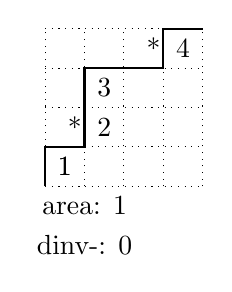
\begin{tikzpicture}[scale=0.5]
\draw[dotted] (0,0) grid (4,4);
\draw[thick] (0,0)--(0,1)--(1,1)--(1,2)--(1,3)--(2,3)--(3,3)--(3,4)--(4,4);
\draw node at (0.5,0.5) {1};
\draw node at (0.500000,0.500000) {1};
\draw node at (1.500000,1.500000) {2};
\draw node at (1.500000,2.500000) {3};
\draw node at (3.500000,3.500000) {4};
\draw node at (0.750000,1.500000) {*};
\draw node at (2.750000,3.500000) {*};
\draw node at (1,-.5) {area: 1};
\draw node at (1,-1.5) {dinv-: 0};
\end{tikzpicture}
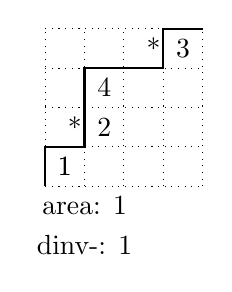
\begin{tikzpicture}[scale=0.5]
\draw[dotted] (0,0) grid (4,4);
\draw[thick] (0,0)--(0,1)--(1,1)--(1,2)--(1,3)--(2,3)--(3,3)--(3,4)--(4,4);
\draw node at (0.5,0.5) {1};
\draw node at (0.500000,0.500000) {1};
\draw node at (1.500000,1.500000) {2};
\draw node at (1.500000,2.500000) {4};
\draw node at (3.500000,3.500000) {3};
\draw node at (0.750000,1.500000) {*};
\draw node at (2.750000,3.500000) {*};
\draw node at (1,-.5) {area: 1};
\draw node at (1,-1.5) {dinv-: 1};
\end{tikzpicture}
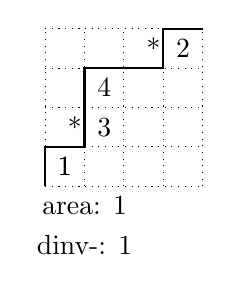
\begin{tikzpicture}[scale=0.5]
\draw[dotted] (0,0) grid (4,4);
\draw[thick] (0,0)--(0,1)--(1,1)--(1,2)--(1,3)--(2,3)--(3,3)--(3,4)--(4,4);
\draw node at (0.5,0.5) {1};
\draw node at (0.500000,0.500000) {1};
\draw node at (1.500000,1.500000) {3};
\draw node at (1.500000,2.500000) {4};
\draw node at (3.500000,3.500000) {2};
\draw node at (0.750000,1.500000) {*};
\draw node at (2.750000,3.500000) {*};
\draw node at (1,-.5) {area: 1};
\draw node at (1,-1.5) {dinv-: 1};
\end{tikzpicture}
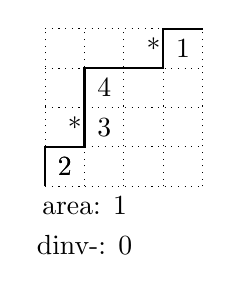
\begin{tikzpicture}[scale=0.5]
\draw[dotted] (0,0) grid (4,4);
\draw[thick] (0,0)--(0,1)--(1,1)--(1,2)--(1,3)--(2,3)--(3,3)--(3,4)--(4,4);
\draw node at (0.5,0.5) {2};
\draw node at (0.500000,0.500000) {2};
\draw node at (1.500000,1.500000) {3};
\draw node at (1.500000,2.500000) {4};
\draw node at (3.500000,3.500000) {1};
\draw node at (0.750000,1.500000) {*};
\draw node at (2.750000,3.500000) {*};
\draw node at (1,-.5) {area: 1};
\draw node at (1,-1.5) {dinv-: 0};
\end{tikzpicture}
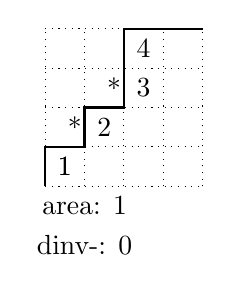
\begin{tikzpicture}[scale=0.5]
\draw[dotted] (0,0) grid (4,4);
\draw[thick] (0,0)--(0,1)--(1,1)--(1,2)--(2,2)--(2,3)--(2,4)--(3,4)--(4,4);
\draw node at (0.5,0.5) {1};
\draw node at (0.500000,0.500000) {1};
\draw node at (1.500000,1.500000) {2};
\draw node at (2.500000,2.500000) {3};
\draw node at (2.500000,3.500000) {4};
\draw node at (0.750000,1.500000) {*};
\draw node at (1.750000,2.500000) {*};
\draw node at (1,-.5) {area: 1};
\draw node at (1,-1.5) {dinv-: 0};
\end{tikzpicture}
\caption{Parking functions of semilength 4 with two marked valleys and area 1.}
\label{fig:val421}
\end{figure}
\end{example}
\end{document}